\section{Auswertung}
\label{sec:Auswertung}

\subsection{Brechender Winkel \texorpdfstring{$\varphi$}{e}}

Der Winkel $\varphi$ berechnet sich nach der Gleichung \ref{eq:varphi} aus den Ablenkungswinkeln der reflektierten Strahlen. Die jeweiligen Messwerte zur Bestimmung des Brechungswinkels befinden sich in der Tabelle \ref{tab:brechungswinkel}.

\begin{table}[htpb]
	\centering
	\caption{Messwerte zur Bestimmung des Brechungwinkels $\varphi$.}
	\label{tab:brechungswinkel}
	\begin{tabular}{c c c}
		\toprule
		$\varphi_\text{r} / ^\circ$ & $\varphi_\text{l} / ^\circ$ & $\varphi / ^\circ$ \\
		\midrule
		204,2 & 84,1 & 60,05 \\
		206 & 86 & 60 \\
		206,9 & 87 & 59,95 \\
		203,9 & 83,8 & 60,05 \\ 
		208 & 88 & 60 \\
		210,1 & 90 & 60,05 \\
		210,7 & 90,8 & 59,95 \\
		\bottomrule
	\end{tabular}
\end{table}

Der Mittelwert $\bar{x}$ aus $n$ Stichproben $x_{i}$ ergibt sich aus:
\begin{equation}
\bar{x}=\frac{1}{n}\sum \limits_{i=1}^n x_{i}
\label{eq:mittelwert}
\end{equation}
Die Standardabweichung errechnet sich nach:
\begin{equation}
\label{eq:standardab}
s_{i}= \sqrt{\frac{1}{n-1}\sum \limits_{i=1}^n(x_{i}-\bar{x})^2}
\end{equation}
mit zufälligen Fehlern behafteten Werten $x_{i}$ mit $i$ = 1,...,n.\\
Der aus der Standardabweichung aus der Gleichung \ref{eq:standardab} resultierende Fehler des Mittelwertes ergibt sich nach:
\begin{equation}
\Delta\bar{x}=\frac{s_{i}}{\sqrt{n}} = \sqrt{\frac{\sum\limits_{i=1}^n(x_{i}-\bar{x})^2}{n(n-1)}}
\label{eq:fehlermittelwert}
\end{equation}

Mit der Gleichung \ref{eq:mittelwert} und \ref{eq:fehlermittelwert} wird nun der Mittelwert sowie der Fehler des Mittelwerts des Brechungswinkels $\varphi$ bestimmt und es ergibt sich der folgende Wert:
\begin{equation*}
\varphi = \SI{60,00 \pm 0,02}{^\circ}.
\end{equation*}

\subsection{Bestimmung des Brechungsindizes n}
Zur Berechnung des Brechungsindizes $n$ wird für jede Wellenlänge $\lambda$ der Brechungswinkel $\eta$ bekannt sein. Der Winkel $\eta$ wird mit der Gleichung \ref{eq:omega} berechnet. Hieraus ergibt sich nach der Gleichung \ref{eq:brechung} die jeweiligen Brechungsindizes $n$. Die Messwerte zu der $\eta$-Messung dazu befinden sich in der Tabelle \ref{tab:brechungswinkel2}.

\begin{table}[htpb]
	\centering
	\caption{Messwerte zur Bestimmung des Brechungindizes $n$.}
	\label{tab:brechungswinkel2}
	\begin{tabular}{c c c c c c}
		\toprule
		$\text{Farbe}$  & $\lambda / \si{\nano\meter}$ & $\Omega_\text{r} / ^\circ$ & $\Omega_\text{l}/ ^\circ$ & $\eta / ^\circ$ & $n$ \\
		\midrule
		rot & 643,84 & 328 & 210,2 & 62,2 & 1,751\\
		orange & 576,96 & 327,5 & 210 & 62,5 & 1,753\\
 		gelb & 546,07 & 327,2 & 211,4 & 64,2 & 1,768\\
		grün & 508,58 & 326,8 & 212 & 65,2 & 1,776\\
		cyan & 479,99 & 326,2 & 212,3 & 66,1 & 1,783\\
 		blau & 467,81 & 326 & 212,6  & 66,6 & 1,787\\
		violett & 453,83 & 325,2 & 213,4 & 68,2 & 1,799\\
 		violett schwach & 404,66 & 324,1 & 214,5 & 70,4 & 1,816\\
		\bottomrule
	\end{tabular}
\end{table}

\subsection{Bestimmung der Dispersionskurve}
Nun soll jetzt überprüft werden, welche der beiden Verläufe aus den Gleichungen \ref{eq:gl11} und \ref{eq:gl12} die Messwerte besser beschreibt. Dazu werden die errechneten Brechungsindizes $n$ aus der Tabelle \ref{tab:brechungswinkel2} quadriert und eine lineare Regression durchgeführt. Die erste Möglichkeit ist gegeben durch die folgende Gleichung:
\begin{equation}
\label{eq:first}
n^{2}(\lambda) = A_0 + \frac{A_2}{\lambda^{2}}.
\end{equation}
Dabei ergibt sich ein linearer Zusammenhang, wenn $n^{2}$ gegen $\frac{1}{\lambda^{2}}$ aufgetragen wird. Die Werte und die errechneten Werte befinden sich in der Abbildung \ref{fig:kurve1}.

\begin{figure}[h!]
	\centering
	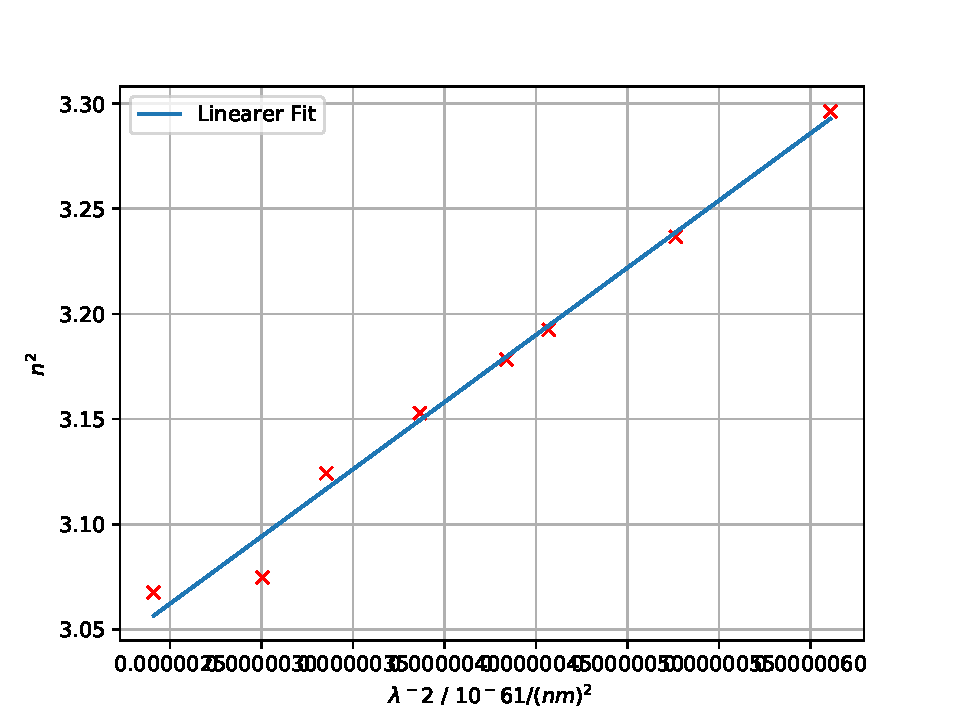
\includegraphics[width=0.9\linewidth]{../../Kurve1}
	\caption{Ausgleichsgerade für die erste Methode.}
	\label{fig:kurve1}
\end{figure}

Eine lineare Ausgleichsgerade lässt sich berechnen wie:
\begin{equation}
\label{eq:ausgleichsgerade}
y = mx + b
\end{equation}
wobei $m$ die Steigung und $b$ der y-Achsenabschnitt sind. Über Formel \ref{eq:ausgleichsgerade} wird die Steigung und der Fehler der Ausgleichsgerade vom Python-Modul Scipy curve\_fit berechnet.
Es ergaben sich für die Ausgleichsgerade $m$ als Steigung und $b$ als y-Achsenabschnitt die folgenden Werte:
\begin{align*}
m &= \SI{63942,4 \pm 3115,3}{\nano\meter^{2}}\\
b &= (2,902 \pm 0,013)
\end{align*}
und somit für $n^{2}$:
\begin{equation*}
n^{2}(\lambda) = (2,902 \pm 0,013) + \frac{\SI{63942,4 \pm 3115,3}{\nano\meter^{2}}}{\lambda^{2}}.
\end{equation*}

Für die zweite Möglichkeit ergibt sich die folgende Gleichung:
\begin{equation}
\label{eq:second}
n'^{2}(\lambda) = A_0' + A_2' \cdot \lambda^{2}.
\end{equation}
Dabei stellt sich ein linearer Zusammenhang fest, wenn $n'^{2}$ gegen $\lambda^{2}$ aufgetragen wird. Die Werte und die errechneten Werte befinden sich in der Abbildung \ref{fig:kurve2}. Analog wird über die Formel \ref{eq:ausgleichsgerade} die Steigung und der Fehler vom Python-Modul Scipy curve\_fit berechnet.

\begin{figure}[h!]
	\centering
	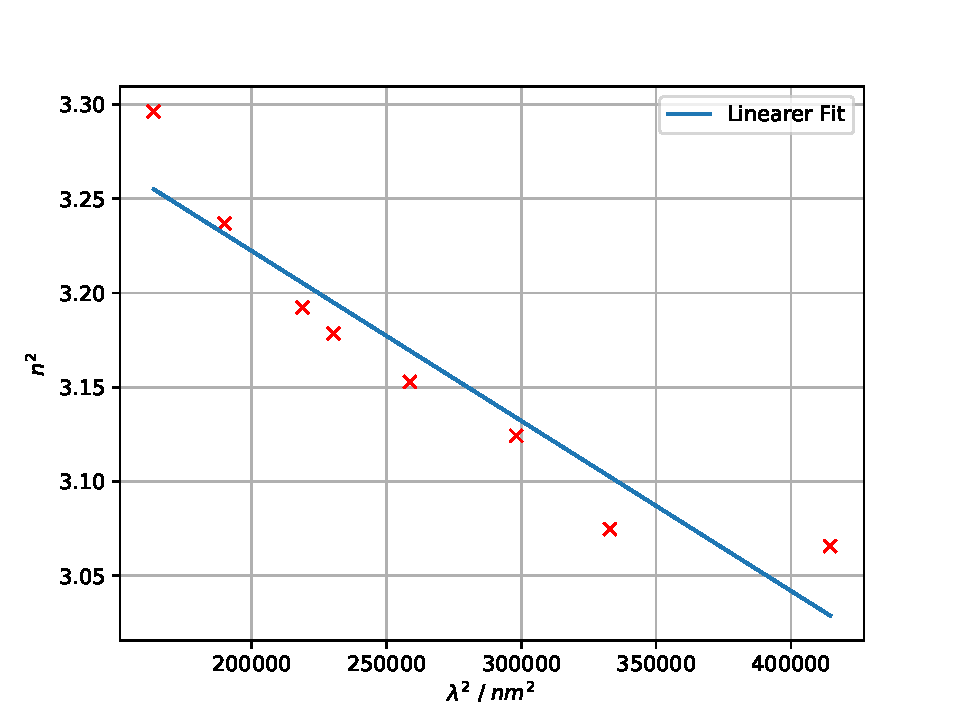
\includegraphics[width=0.9\linewidth]{../../Kurve2}
	\caption{Ausgleichsgerade für die zweite Methode.}
	\label{fig:kurve2}
\end{figure}

Es ergaben sich für die Ausgleichsgerade $m$ als Steigung und $b$ als y-Achsenabschnitt die folgenden Werte:
\begin{align*}
m &= \SI{-9,01\pm 1,28 e-7}{\frac{1}{\nano\meter^{2}}}\\
b &= (3,402 \pm 0,035)
\end{align*}
und somit für $n'^{2}$:
\begin{equation*}
n'^{2}(\lambda) = (3,402 \pm 0,035) + \SI{9,01\pm 1,28 e-7}{\frac{1}{\nano\meter^{2}}} \cdot \lambda^{2}.
\end{equation*}

Zum Vergleich der beiden Möglichkeiten wird die Summe der Abweichungsquadrate benötigt:
\begin{equation}
\label{eq:abw1}
s_\text{n}^2 = \frac{1}{z-2} \sum_{i=1}^{z}   \left(n^2(\lambda_\text{i}) - A_0 -\frac{A_2}{\lambda_\text{i}^2}\right)^2
\end{equation}
und 
\begin{equation}
\label{eq:abw2}
s_\text{n'}^2 = \frac{1}{z-2} \sum_{i=1}^{z}   \left(n^2(\lambda_\text{i}) - A_0' + A_2'\lambda_\text{i}^2\right)^2,
\end{equation}
wobei $z$ die Anzahl der Messungen ist. Für die erste Möglichkeit nach der Gleichung \ref{eq:abw1} ergibt sich ein Wert von:
\begin{equation*}
s_\text{n}^2 = 9,413 \cdot 10^{-5}
\end{equation*}
und für die zweite Möglichkeit nach der Gleichung \ref{eq:abw2} ergibt sich:
\begin{equation*}
s_\text{n'}^2 = 0,326.
\end{equation*}
Es ergibt sich, dass die Abweichungsquadrate der ersten Dispersionsgleichung kleiner sind als die der zweiten. Zum einen lautet die Dispersionsgleichung wie folgt:
\begin{equation}
\label{eq:dispersionsgleichung}
n(\lambda) = \sqrt{(2,902 \pm 0,013) + \frac{\SI{63942,4 \pm 3115,3}{\nano\meter^{2}}}{\lambda^{2}}}
\end{equation}
und zum anderen ist diese Gleichung zusammen mit den errechneten Werten in die Abbildung \ref{fig:dispersionskurve}  dargestellt.
\begin{figure}[h!]
	\centering
	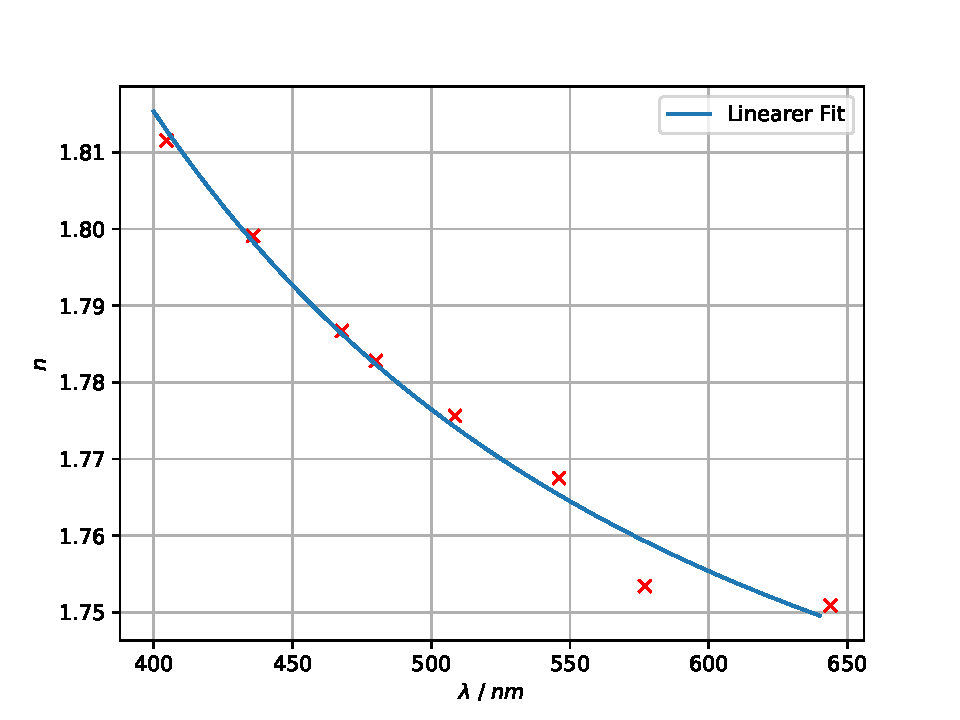
\includegraphics[width=0.9\linewidth]{../../Dispersionskurve}
	\caption{Die Dispersionskurve mit den errechneten Werten.}
	\label{fig:dispersionskurve}
\end{figure}

\subsection{Bestimmung der Abbeschen Zahl}
Im nächsten Aufgabenteil soll die Abbesche Zahl aus der bestimmten Dispersionsgleichung ausgerechnet werden. Dafür wird die vorherige Gleichung \ref{eq:dispersionsgleichung} verwendet. Es werden die drei Frauenhoferschen Linien mit $\lambda_\text{C}= \SI{656}{\nano\meter}$, $\lambda_\text{D} = \SI{589}{\nano\meter}$ und $\lambda_\text{F} = \SI{486}{\nano\meter}$ eingesetzt und es ergaben sich die folgenden Brechungsindizes:
\begin{align*}
n_\text{C} &= 1,746 \\
n_\text{D} &= 1,757 \\
n_\text{F} &= 1,781.
\end{align*}
Es muss eine Fehlerfortpflanzung durchgeführt werden, da die Brechungsindizes aus den fehlerbehafteten Größen $A_0$ und $A_2$ bestimmt worden sind. Die Fehlerfortpflanzung ist im Allgemeinen gegeben durch:
\begin{equation}
\label{eq:gaußallg}
\sigma_\text{f} = \sqrt{\sum_{i=1}^{n} \left(\frac{\partial g}{\partial y_i}\right)^2 (\sigma_y)^2}
\end{equation}
wobei $\sigma_f$ der Fehler ist, der zu errechnenden Größe $f$, die aus den fehlerbehafteten Größen $y_\text{i}$ mit den jeweiligen Fehlern $\sigma_y$ mit der Formel $f$ berechnet wird. Also in dem Fall wird der Fehler berechnet durch:
\begin{equation}
\label{eq:fehlergauß}
\sigma_\text{n} = \sqrt{\left(\frac{1}{2\sqrt{A_0+\frac{A_2}{\lambda^2}}}\right)^2 \cdot \sigma^2_{A_0} + \left(\frac{1}{2 \lambda^2 \sqrt{A_0 + \frac{A_2}{\lambda^2}}}\right)^2 \cdot \sigma^2_{A_2}}.
\end{equation}
Für die jeweiligen Brechungsindizes $n$ ergeben sich die folgenden Fehler:
\begin{align*}
\sigma_{n_C} &= 0,004 \\
\sigma_{n_D} &= 0,0045 \\
\sigma_{n_F} &= 0,005.
\end{align*}
Letztendlich für die Abbesche Zahl wird die folgende Gleichung benötigt:
\begin{equation}
\label{eq:abbesche}
\nu = \frac{n_\text{D}-1}{n_\text{F} - n_\text{C}}
\end{equation}
und dafür ergibt sich ein Wert, bei dem auch die Fehler fortgepflanzt wird, von:
\begin{equation*}
\nu = 21,62 \pm 3,95.
\end{equation*}

\subsection{Das theoretische Auflösungsvermögen}
Im nächsten Teil soll das theoretische Auflösungsvermögen bestimmt werden unter der Annahme, dass das Prisma voll ausgeleuchtet ist. Bei voller Ausleuchtung ergibt sich das Auflösungsvermögen $A$ zu:
\begin{equation}
\label{eq:aufl}
A = \frac{\lambda}{\Delta \lambda} = b\frac{dn}{d\lambda},
\end{equation}
wobei $\lambda$ die Wellenlänge und $\Delta \lambda$ den kleinsten messbaren Wellenlängenunterschied zweier benachbarter Spektrallinien darstellt und mit der Ableitung der Dispersionsgleichung nach $\lambda$ ergibt sich dann auch zu:
\begin{equation}
\frac{dn}{d\lambda} = - \frac{A_2}{\lambda^3 \sqrt{A_0 +\frac{A_2}{\lambda^2}}}.
\end{equation}
Analog werden hier die vorherigen Frauenhofscher Linien $\lambda_\text{C}$ und $\lambda_\text{F}$, die Basislänge $b = \SI{3}{\cm}$ und in die Gleichung \ref{eq:aufl} eingesetzt:
\begin{align*}
A_\text{C} &= 3890,5 \\
A_\text{F} &= 9381,7.
\end{align*}
Der Fehler berechnet sich erneut nach der Gleichung \ref{eq:gaußallg} wie folgt:
\begin{equation}
\sigma_A = \sqrt{\left(\frac{bA_2}{2\lambda^3(A_0+\frac{A_2}{\lambda^2})^{\frac{3}{2}}}\right)^2 \cdot \sigma^2_{A_0} + \left(\frac{-b}{\lambda^3\sqrt{A_0+\frac{A_2}{\lambda^2}}}+\frac{bA_2}{2\lambda^5(A_0+\frac{A_2}{\lambda^2})^{\frac{3}{2}}} \right)^2 \cdot \sigma^2_{A_2}} 
\end{equation}
und die Fehler betragen dann:
\begin{align*}
\sigma_{A_C} &= 185,53 \\
\sigma_{A_F} &= 439,03
\end{align*}
Insgesamt ergibt sich ein Auflösungsvermögen von:
\begin{align*}
A_C &= 3890,5 \pm 185,53 \\
A_F &= 9381,7 \pm 439,03.
\end{align*}

\subsection{Bestimmung der Absorptionsstelle}
Nun soll die dem sichtbaren Bereich am nächsten liegende Absorptionsstelle $\lambda_1$ berechnet werden. 
Für die Bestimmung der Absorptionsstelle, gelten die folgenden Formeln:
\begin{align}
n^2(\lambda) &= 1+ \frac{N_1 q^2_1 \lambda^2_1}{4 \pi^2 c^2 \epsilon_0 m_1} \left(1+ \left(\frac{\lambda_1}{\lambda}\right)^2 \right) \\
n^2(\lambda) &= A_0 + \frac{A_2}{\lambda^2}.
\end{align}
Dabei sind $A_0$ und $A_2$ gegeben wie folgt:
\begin{align}
A_0 &= 1 + \frac{N_1 q^2_1 \lambda^2_1}{4 \pi^2 c^2 \epsilon_0 m_1} \\
A_2 &= \lambda^2_1(A_0 - 1)
\end{align}
und diese beiden Gleichungen müssen entsprechend nun nach $\lambda_1$ aufgelöst werden, welches ja die gesuchte Wellenlänge der nächsten Absorptionsstelle darstellt:
\begin{align*}
\lambda_1 &= \sqrt{\frac{A_2}{A_0-1}} \\
\lambda_1 &= \SI{183,25}{\nano\meter}.
\end{align*}